\section{Benutzeroberfläche}

Die folgenden Abschnitte beschreiben die Benutzeroberfläche von \textbf{JExam} anhand der bereitgestellten UI-Bilder. Jede Abbildung wird durch einen erklärenden Text ergänzt, der beschreibt, welche Funktion dort ausgeführt wird und in welchem Kontext das Element genutzt wird.

Hinweis: Die Tatsächliche UI der Anwendung \textbf{JExam} kann leicht von der Hier beschriebenen Benutzeroberfläche abweichen. Die Struktur und wo was ist bleiben Identisch.

% ============================================================
\subsection{Navigation}

\subsubsection*{Header Navigation}
Der Header ermöglicht das Umschalten zwischen der XML-Strukturansicht und der PDF-Konfiguration.
\begin{figure}[H]
    \vspace{0pt}
    \centering
    \includegraphics[scale=0.5]{fig/header.pdf}
    \caption{Navigation zwischen XML- und PDF-Modus.}
\end{figure}

\subsubsection*{Breadcrumbs}
Die Breadcrumb-Leiste dient zur Navigation auf der aktuellen Hierarchieebene. Sie zeigt den Pfad zum aktuell ausgewählten Objekt (Exam → Chapter → Task).
\begin{figure}[H]
    \vspace{0pt}
    \centering
    \includegraphics[scale=0.5]{fig/breadcrumbs.pdf}
    \caption{Navigation innerhalb der aktuellen Objektstruktur.}
\end{figure}

\begin{figure}[H]
\centering
\begin{minipage}[t]{0.55\linewidth}
    \vspace{0.5em}

    \subsubsection*{TreeView}

    Der TreeView zeigt die gesamte XML-Struktur (Exam → Chapter → Task). 

    Über Dropdowns kann jede Ebene ein- und ausgeklappt werden.  

    Ist noch kein Exam vorhanden, erscheint ein \textit{Create Exam}-Button, der das entsprechende Popup öffnet.
\end{minipage}
\hfill
\begin{minipage}[t]{0.40\linewidth}
    \vspace{0pt}
    \centering
    \includegraphics[scale=0.5]{fig/treeview.pdf}
    \caption{Navigation zwischen allen Objekten der XML-Datei.}
\end{minipage}
\end{figure}


% ============================================================
\subsection{Komponenten}

\subsubsection*{Chapter Component}
Eine Anzeige des Kapitels mit Buttons zum Bearbeiten oder Löschen. Löschen öffnet ein Popup und Bearbeiten navigiert in die Chapter Seite.
\begin{figure}[H]
    \vspace{0pt}
    \centering
    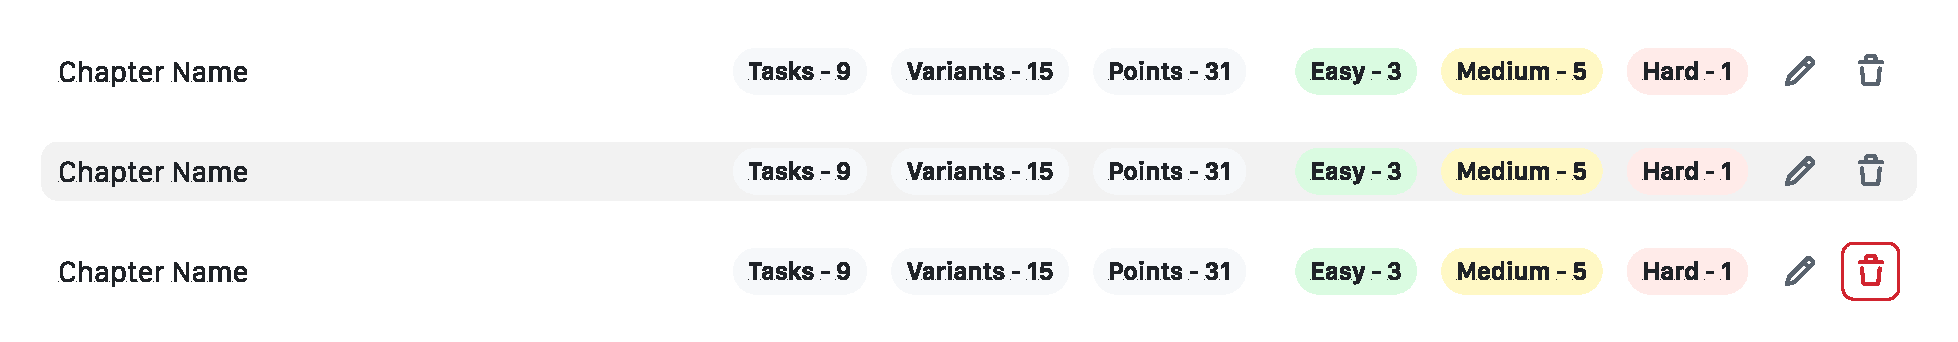
\includegraphics[scale=0.5]{fig/chapter_component.pdf}
    \caption{Chapter Component mit Edit- und Delete-Optionen.}
\end{figure}

\subsubsection*{Task Component}
Ein Task wird mit Punktzahl, Schwierigkeit und Sichtbarkeit dargestellt. Enthält Edit- und Delete-Aktionen. Löschen öffnet ein Popup und Bearbeiten navigiert in die Chapter Seite.
\begin{figure}[H]
    \vspace{0pt}
    \centering
    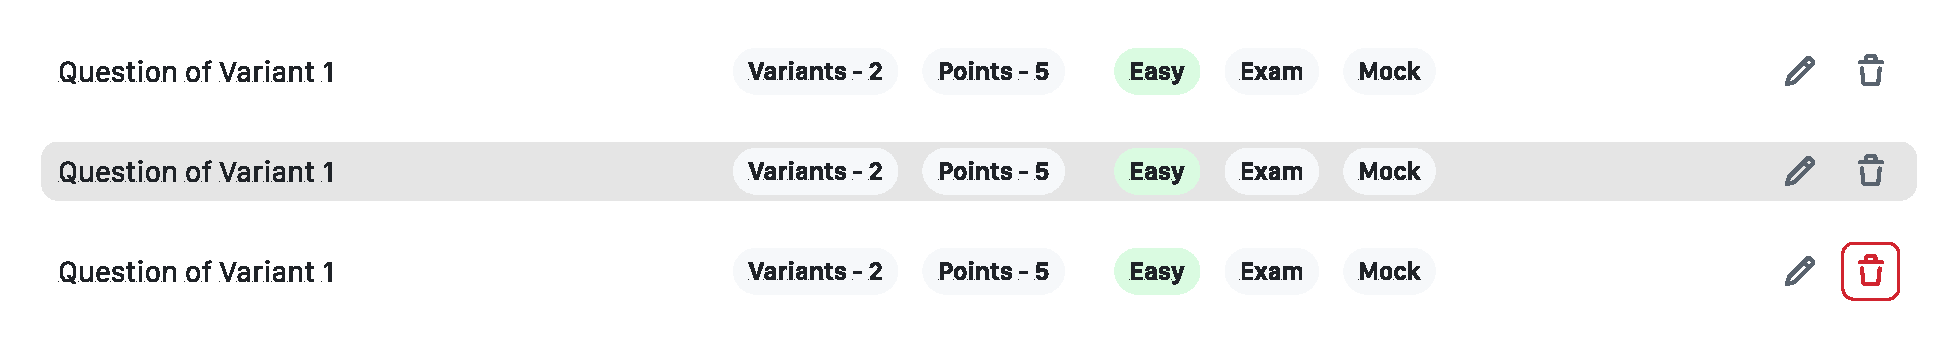
\includegraphics[scale=0.5]{fig/task_component.pdf}
    \caption{Task Component mit Bearbeitungs- und Löschmöglichkeiten.}
\end{figure}

\subsubsection*{Variant Component}
Zeigt Frage und Antwort einer Variante an und bietet Textfelder um die Fragen und Antworten zu bearbeiten und den Delete Button, welcher ein Popup öffnet.
\begin{figure}[H]
    \vspace{0pt}
    \centering
    \includegraphics[scale=0.5]{fig/variant_component.pdf}
    \caption{Variant Component zur Bearbeitung einzelner Varianten.}
\end{figure}

% ============================================================
\subsection{Exam ausgewählt}

\begin{figure}[H]
\centering
\begin{minipage}[t]{0.55\linewidth}
    \vspace{0pt}
    \subsubsection*{Exam Header}

    Ermöglicht das Umbenennen des Exams.
\end{minipage}
\hfill
\begin{minipage}[t]{0.40\linewidth}
    \vspace{0pt}
    \centering
    \includegraphics[scale=0.5]{fig/exam_header.pdf}
    \caption{Exam Header zur Anpassung des Exam-Namens.}
\end{minipage}
\end{figure}


\subsubsection*{Chapter Table}
Zeigt alle bestehenden Chapter Components an.  
Ein \textit{Create Chapter}-Button öffnet das Kapitel-Erstellungs-Popup.
\begin{figure}[H]
    \vspace{0pt}
    \centering
    \includegraphics[scale=0.5]{fig/chapter_table.pdf}
    \caption{Tabelle aller Kapitel mit Option zur Neuerstellung.}
\end{figure}

% ============================================================
\subsection{Chapter ausgewählt}

\begin{figure}[H]
\centering
\begin{minipage}[t]{0.55\linewidth}  % Text oben ausgerichtet
    \vspace{0pt}
    \subsubsection*{Chapter Header}

    Ermöglicht das Umbenennen sowie das Löschen eines Kapitels.  
    Der Delete-Button öffnet die Bestätigungsabfrage.
\end{minipage}
\hfill
\begin{minipage}[t]{0.40\linewidth}  % Bild ebenfalls oben ausgerichtet
    \vspace{0pt}
    \centering
    \includegraphics[scale=0.5]{fig/chapter_header.pdf}
    \caption{Header eines Kapitels mit Edit- und Delete-Funktionen.}
\end{minipage}
\end{figure}


\subsubsection*{Task Table}
Die Tabelle zeigt alle Tasks des Kapitels.  
Mit dem Button \textit{Create Task} wird das Task-Erstellungs-Popup geöffnet.
\begin{figure}[H]
    \vspace{0pt}
    \centering
    \includegraphics[scale=0.5]{fig/task_table.pdf}
    \caption{Tabelle aller Tasks eines Kapitels.}
\end{figure}

% ============================================================
\subsection{Task ausgewählt}

\begin{figure}[H]
\centering
\begin{minipage}[t]{0.55\linewidth}  % Text oben ausgerichtet
    \vspace{0pt}
    \subsubsection*{Task Header}

    Hier können die Eigenschaften des Tasks angepasst werden:  
    Scope (\texttt{mock/exam}), Difficulty (\texttt{easy/medium/hard}) und Punktzahl.  
    Der Delete-Button öffnet das Lösch-Popup.
\end{minipage}
\hfill
\begin{minipage}[t]{0.40\linewidth}  % Bild ebenfalls oben ausgerichtet
    \vspace{0pt}
    \centering
    \includegraphics[scale=0.5]{fig/task_header.pdf}
    \caption{Header eines Tasks mit konfigurierbaren Eigenschaften.}
\end{minipage}
\end{figure}

\pagebreak
\subsubsection*{Variant List}
Eine Liste aller Varianten des Tasks.  
Der \textit{Create Variant}-Button öffnet das entsprechende Popup.
\begin{figure}[H]
    \vspace{0pt}
    \centering
    \includegraphics[scale=0.5]{fig/variant_list.pdf}
    \caption{Variantenliste zur Verwaltung aller Varianten eines Tasks.}
\end{figure}

% ============================================================
\subsection{PopUp}

\begin{figure}[H]
\centering
\begin{minipage}[t]{0.55\linewidth}
    \vspace{0.5em}

    \subsubsection*{Delete Popup}

    Popup zur Bestätigung des Löschens eines Class (ersetzen durch Chapter, Task, Variant).
    Gibt die Bedeutung zurück, dass auch alle Kindelemente unwiderruflich gelöscht werden.
\end{minipage}
\hfill
\begin{minipage}[t]{0.40\linewidth}
    \vspace{0pt}
    \centering
    \includegraphics[scale=0.5]{fig/delete_popup.pdf}
    \caption{Löschbestätigung für Class}
\end{minipage}
\end{figure}

\subsection{Rearrange Chapters}

\begin{figure}[H]
\centering
\begin{minipage}[t]{0.4\linewidth}
    \vspace{0.5em}

    \subsubsection*{Rearrange Chapters \& Create Exam}

    Ermöglicht die Reihenfolge der Chapter für die Klausurgenerierung zu ändern.

    Durch Verschieben in den "Excluded from PDF Generation" Bereich werden diese Chapter nicht mehr für die Generierung berücksichtigt und somit ausgeschlossen.
\end{minipage}
\hfill
\begin{minipage}[t]{0.55\linewidth}
    \vspace{0pt}
    \centering
    \includegraphics[scale=0.5]{fig/pdf_sidebar.pdf}
    \caption{Umordnen der Chapters}
\end{minipage}
\end{figure}

